\chapter{Experiments} % Results

This chapter presents simulation scenarios chosen to demonstrate the performance and limitations of the simulator, and to show the concept of OAL.

A common configuration for all experiments is given in table \ref{tab:var-allcases}. The individual configurations are presented in the respective sections.

\begin{table}
\centering
    \begin{tabular}{|c|c|c|}
        \hline
         \textbf{Description} & \textbf{Variable name} & \textbf{Value} \\
         \hline
         Link length $[m]$& \texttt{l} & $1$ \\
         \hline
         Link mass $[kg]$& \texttt{m} & $1$ \\
         \hline
         Obstacle safety radius $[m]$& \texttt{obstacle\char`_radius} & $0.1$\\
         \hline
    \end{tabular}
    \caption{Common simulation configuration for all cases}
    \label{tab:var-allcases}
\end{table}



%---------------------------------------------------------------------------------------
%---------------------------------------------------------------------------------------
%---------------------------------------------------------------------------------------

\section{Obstacle-free environment}

This section briefly demonstrates how the robot behaves without the influence of obstacles in the environment.

\subsection{Case 1.1: Single reference computed torque control}

This case is to demonstrate two damping modes of the computed torque controller in a simple scenario. The configurations for the experiment are summarized in table \ref{tab:var-case-1-1}.

\begin{table}
\centering
    \begin{tabular}{|c|c|c|}
        \hline
         \textbf{Description} & \textbf{Variable name} & \textbf{Value} \\
         \hline
         Simulation time $[s]$& \texttt{simTime} & $30$ \\
         \hline
         Simulation sample time $[s]$& \texttt{h} & $0.01$ \\
         \hline
         Number of links & \texttt{n} & $4$ \\
         \hline
         Joint angle setpoints $[rad]$ & \texttt{q\char`_ref} & $[0, \pi/2, -\pi/3, -\pi/2]$ \\
         \hline
         Initial joint angles $[rad]$ & \texttt{q\char`_0(1:n)} & $[0, 0, 0, 0]$ \\
         \hline
         Initial position $[m]$ & \texttt{q\char`_0(n+1:n+2)} & $[0, 0]$ \\
         \hline
    \end{tabular}
    \caption{Simulation configuration for case 1.1}
    \label{tab:var-case-1-1}
\end{table}


Figure \ref{fig:case1-1} shows the different damping-cases using the computed torque controller for following joint angle references. These references are plotted as dashed lines. Please note that the joint angle $q_1 = \phi_1$ is not included as it is a virtual coordinate and not directly actuated.

The critically damped configuration with $\zeta = 1$ is mainly used throughout the experiments. The overdamped case with $\zeta=2$ is used only when very slow motions is desired to avoid abrupt movement. The underdamped case is not relevant for this project and left out.

The proportional gain is chosen to be $\mathbf{K_p} = 0.4 \mathbf{I}$ in all cases. The relation in (\ref{eq:control2}) with $\zeta=1$ and $\zeta=2$ yields $\mathbf{K_d} = 1.3 \mathbf{I}$ and $\mathbf{K_d} = 2.5 \mathbf{I}$ respectively.

\begin{figure}
    \centering

    \subfloat[Critically damped]{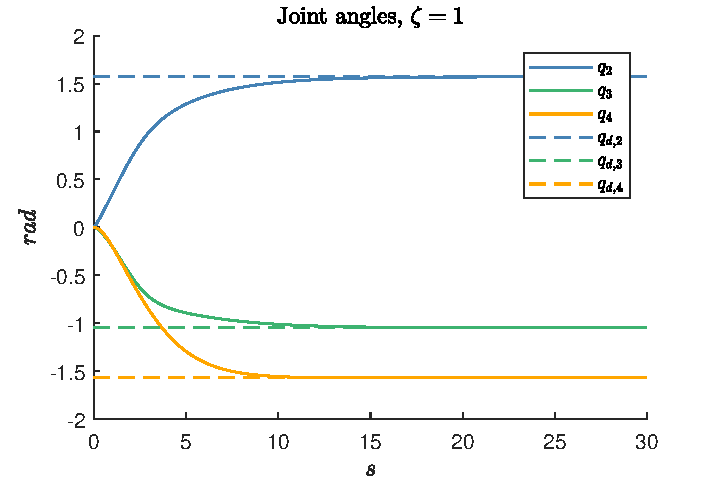
\includegraphics[totalheight=0.4\textheight]{figures/case-1-1/control-critdamped.pdf}}

    \subfloat[Overdamped]{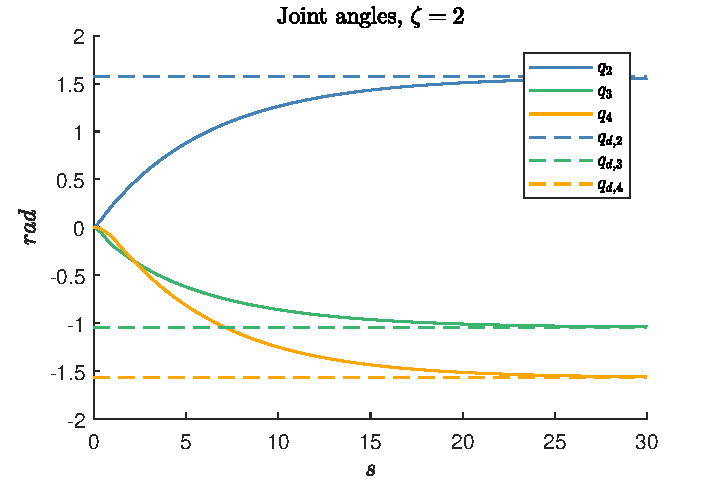
\includegraphics[totalheight=0.4\textheight]{figures/case-1-1/control-overdamped.pdf}}

    \caption{Simulation demo - computed torque control}
    \label{fig:case1-1}
\end{figure}


%---------------------------------------------------------------------------------------
%---------------------------------------------------------------------------------------

\subsection{Case 1.2: Path alignment}\label{subseq:case12}

In this case, the robot is initialized with two different start positions before attempting to adjust to the same path (\ref{eq:path}), which consists of line segments and quadrants. The variable configurations are summarized in table \ref{tab:var-case-1-2}.

The figures \ref{fig:case1-2a} and \ref{fig:case1-2b} show the start and end position of the adjustment in a 15 second interval. It is evident that path adjustment relies on a start configuration close to the path to be successful. However, none of the simulations are able to perfectly adjust to the path. An important reason for this is that the robot cannot change the position of its center of mass without friction or push-points (obstacles) in the environment.

The plots in figure \ref{fig:case1-2-plot} show the joint angles of the controllable joints during the simulations. The reference angles are plotted with a dashed line. It can be observed that he end effector is very close to the path and the corresponding reference angles $q_{d,4}$ are almost met in both cases. Additionally, the reference angles of link 2 and 3 wish to bend the links downward to the path. This is logical, just not completely feasible. A consequence of this is that the robot too far from the path is curling up. The projection method is not considering that the snake robot should be stretched out along the path at all times.

\begin{equation}\label{eq:path}
    y(x) =
    \begin{cases}
        0, & \text{if } x < 2.2 \\
        \sqrt{4 - (x - 2.2)^2} + 2, & \text{if } x \in [2.2, 4.2] \\
        -\sqrt{4 - (x - 6.2)^2} + 2, & \text{if } x \in [4.2, 6.2] \\
        -4, & \text{if } x > 6.2
    \end{cases}
\end{equation}


\begin{table}
\centering
    \begin{tabular}{|c|c|c|}
        \hline
         \textbf{Description} & \textbf{Variable name} & \textbf{Value} \\
         \hline
         Simulation time $[s]$& \texttt{simTime} & $15$ \\
         \hline
         Simulation sample time $[s]$& \texttt{h} & $0.001$ \\
         \hline
         Damping ratio & \texttt{zeta} & $2$ \\
         \hline
         Number of links & \texttt{n} & $4$ \\
         \hline
         Joint angle setpoints $[rad]$ & \texttt{q\char`_ref} & From path \\
         \hline
         Initial joint angles $[rad]$ & \texttt{q\char`_0(1:n)} & $[0, 0, 0, 0]$ \\
         \hline
         \makecell{Initial position part 1 $[m]$\\Initial position part 2 $[m]$} & \texttt{q\char`_0(n+1:n+2)} & \makecell{$[0, 0]$ \\ $[0, -1]$} \\
         \hline
    \end{tabular}
    \caption{Simulation configuration for case 1.2}
    \label{tab:var-case-1-2}
\end{table}


\begin{figure}
    \centering
    
    \subfloat[$t = 0 s$]{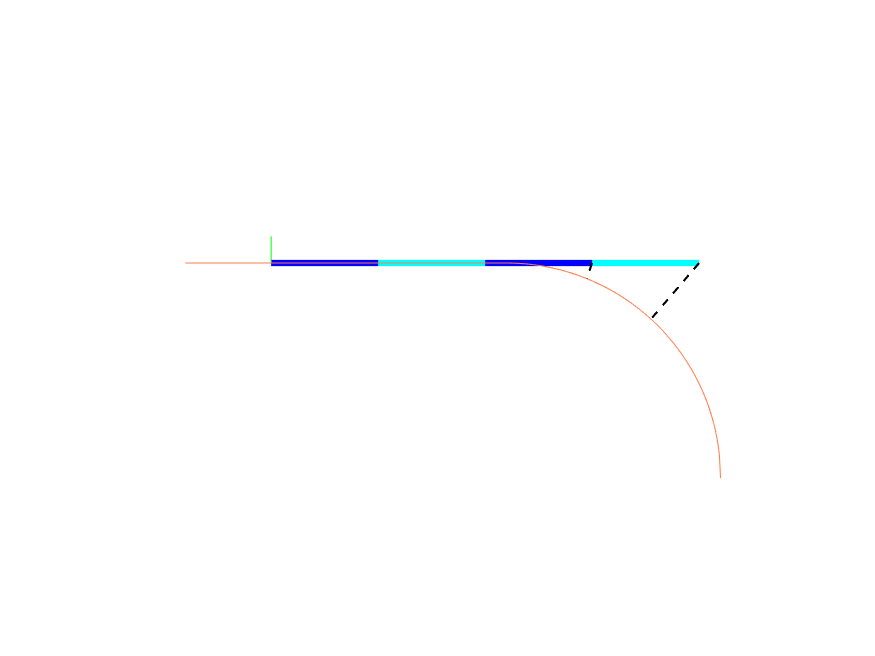
\includegraphics[trim=2cm 2cm 2cm 2cm, clip=true, totalheight=0.23\textheight] {figures/case-1-2/goodgirl1.png}}
    \hfil
    \subfloat[$t = 15 s$]{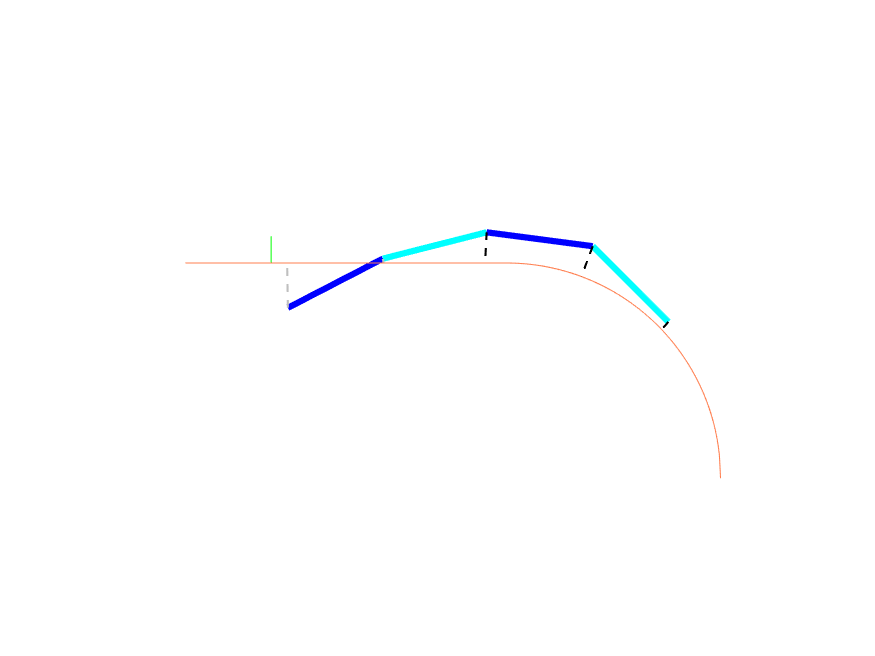
\includegraphics[trim=2cm 2cm 2cm 2cm, clip=true, totalheight=0.23\textheight]{figures/case-1-2/goodgirl3.png}}
    
    \caption{Simulation demo - adjusting to path from nearby}
    \label{fig:case1-2a}
\end{figure}

\begin{figure}
    \centering
    
    \subfloat[$t = 0 s$]{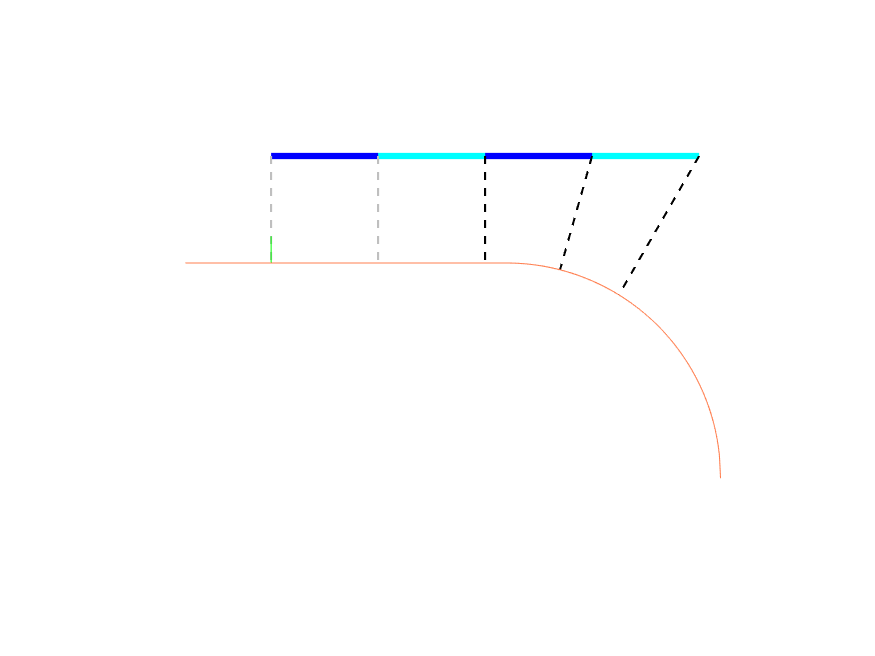
\includegraphics[trim=2cm 2cm 2cm 2cm, clip=true, totalheight=0.23\textheight] {figures/case-1-2/badgirl1.png}}
    \hfil
    \subfloat[$t = 15 s$]{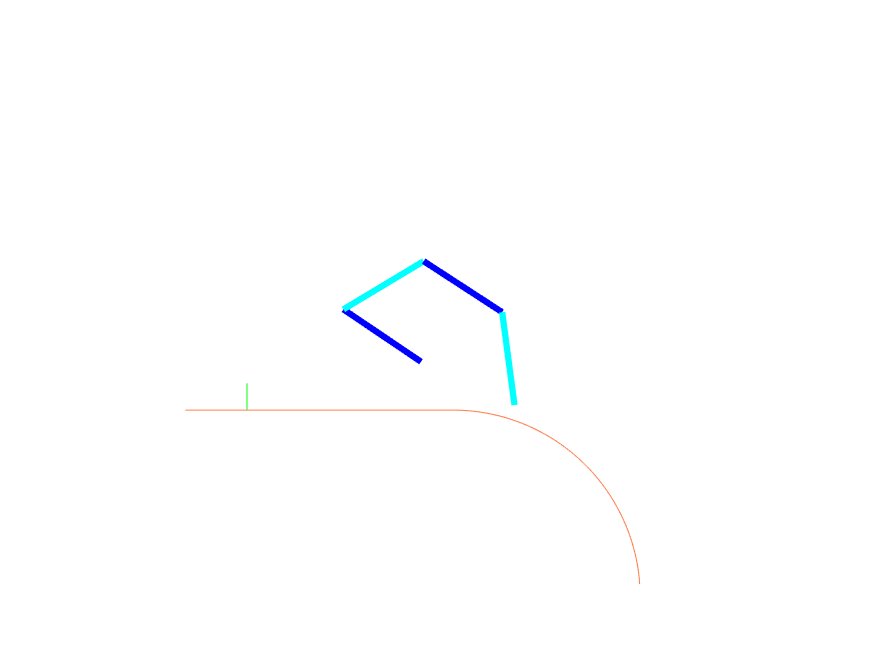
\includegraphics[trim=2cm 2cm 2cm 2cm, clip=true, totalheight=0.23\textheight]{figures/case-1-2/badgirl3.png}}
    
    \caption{Simulation demo - adjusting to path from a distance}
    \label{fig:case1-2b}
\end{figure}

\begin{figure}
    \centering
    
    \subfloat[Start at $(x_0,y_0) = (0,0)$]{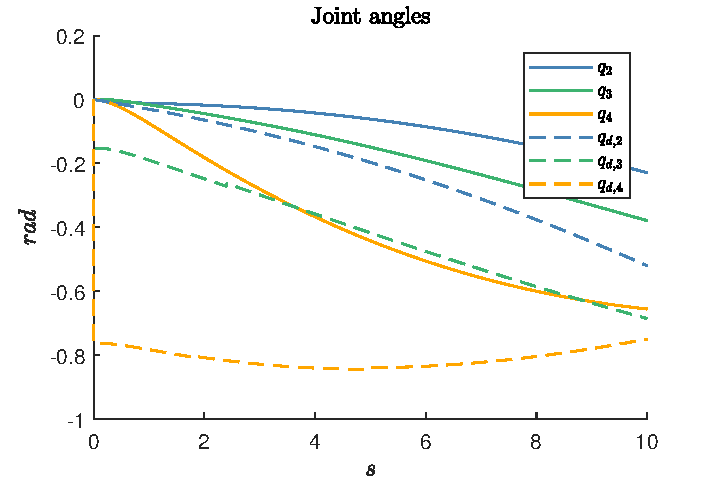
\includegraphics[clip=true, totalheight=0.39\textheight]{figures/case-1-2/case12a.pdf}}

    \subfloat[Start at $(x_0,y_0) = (0,-1)$]{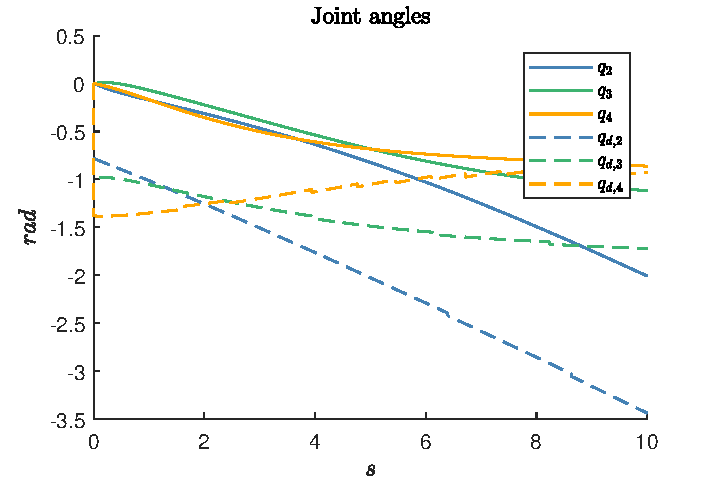
\includegraphics[clip=true, totalheight=0.39\textheight]{figures/case-1-2/case12b.pdf}}

    \caption{Joint angles for path adjustment with different starting configurations}
    \label{fig:case1-2-plot}
\end{figure}

%---------------------------------------------------------------------------------------
%---------------------------------------------------------------------------------------
%---------------------------------------------------------------------------------------

\section{OAL simulation scenarios}

\subsection{Case 2.1: Simple propulsion}\label{subseq:case21}

This scenario aims a demonstrating the concept of OAL. The snake robot is simply set to bend its front joint to $-\pi/2$ while the other joints are to remain in a stretched out configuration. The simulator variable configuration can be seen in table \ref{tab:var-case-2-1}.
\begin{table}
\centering
    \begin{tabular}{|c|c|c|}
        \hline
         \textbf{Description} & \textbf{Variable name} & \textbf{Value} \\
         \hline
         Simulation time $[s]$& \texttt{simTime} & $20$ \\
         \hline
         Simulation sample time $[s]$& \texttt{h} & $0.001$ \\
         \hline
         Damping ratio & \texttt{zeta} & $2$ \\
         \hline
         Number of links & \texttt{n} & $4$ \\
         \hline
         Joint angle setpoints $[rad]$ & \texttt{q\char`_ref} & $[0, 0, 0, -\pi/2]$ \\
         \hline
         Initial joint angles $[rad]$ & \texttt{q\char`_0} & $[0, 0, 0, 0]$ \\
         \hline
         Number of obstacles & \texttt{num\char`_obstacles} & $3$ \\         
         \hline
         Obstacle positions $[m]$& \texttt{obstacle\char`_coords} & \makecell{$(0.8, -0.08)$ \\ $(1.6, 0.08)$ \\ $(3.3, -0.3)$} \\
         \hline
    \end{tabular}
    \caption{Simulation configuration for case 2.1}
    \label{tab:var-case-2-1}
\end{table}

The setpoints are manually set based on the knowledge that the bending link will collide with an obstacle in trying to fulfill the task. In order to obtain the desired angle, the link will apply a force to the obstacle underneath and consequently drag the whole robot body in the positive $x$ (rightward) direction. A sequence of the movement is presented in figure \ref{fig:case2-1}. The obstacles laying close to the rear links are positioned to allow the rest of the robot to stay flat. From the figure it can be seen that the robot moves away from the obstacles towards the end without pushing against anything. This is a consequence of the modeled frictionless environment.

\begin{figure}
    \centering
    
    \subfloat[$t = 0 s$]{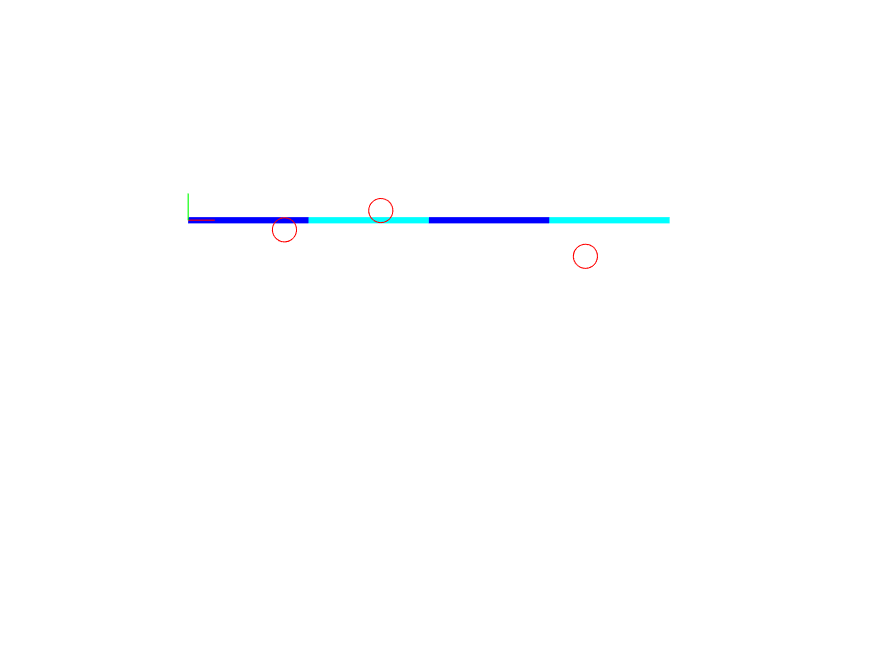
\includegraphics[trim=2cm 4cm 2cm 1.5cm, clip=true, totalheight=0.18\textheight] {figures/case-2-1/sim1.png}}
    \hfil
    \subfloat[$t = 4 s$]{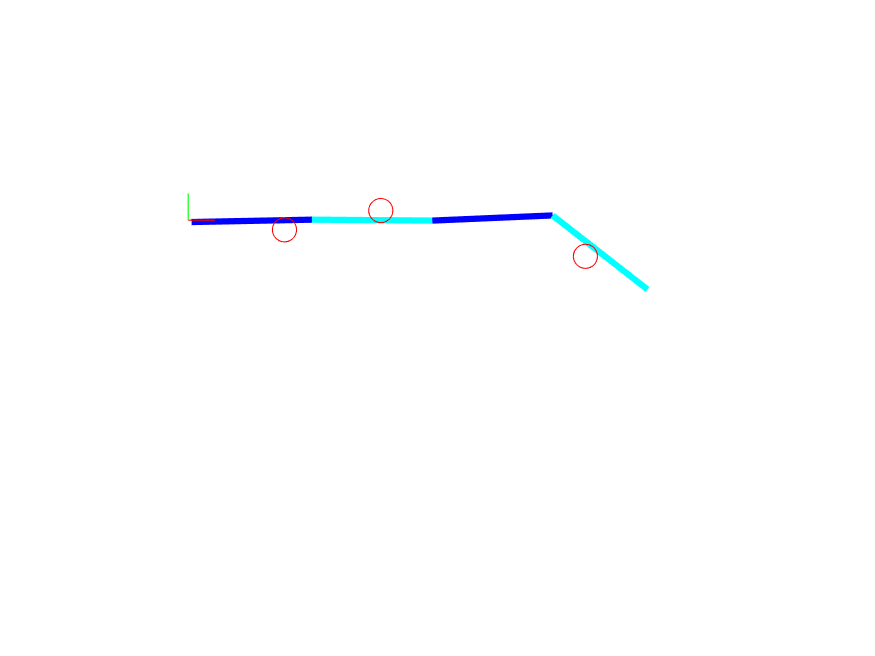
\includegraphics[trim=2cm 4cm 2cm 1.5cm, clip=true, totalheight=0.18\textheight]{figures/case-2-1/sim2.png}}
    
    \subfloat[$t = 8 s$]{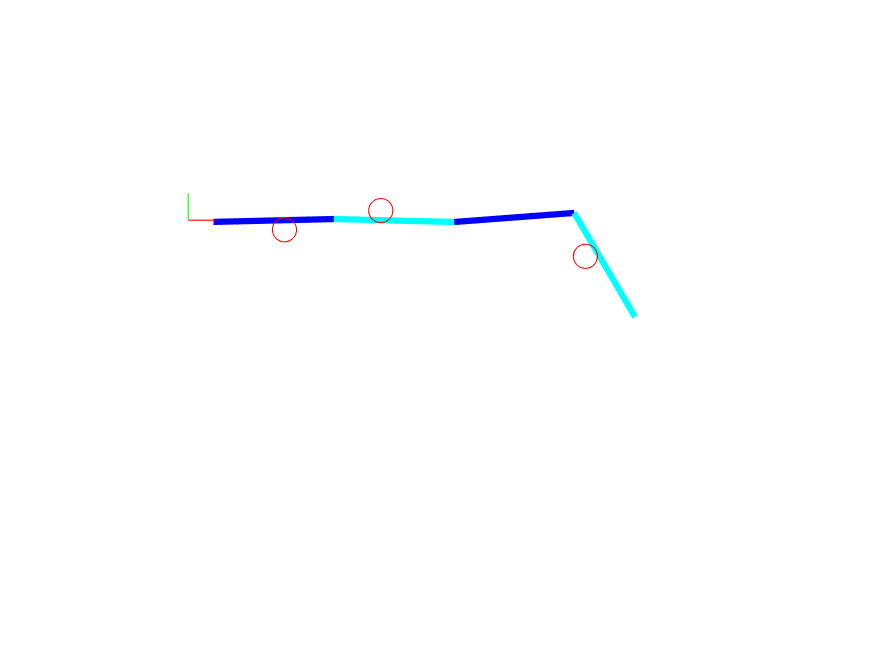
\includegraphics[trim=2cm 4cm 2cm 1.5cm, clip=true, totalheight=0.18\textheight]{figures/case-2-1/sim3.png}}
    \hfil
    \subfloat[$t = 12 s$]{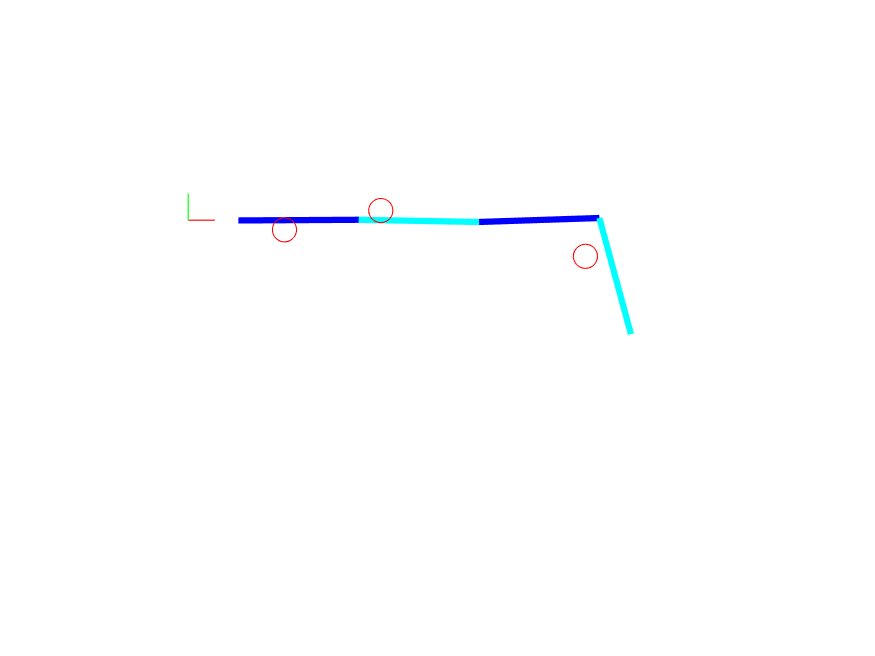
\includegraphics[trim=2cm 4cm 2cm 1.5cm, clip=true, totalheight=0.18\textheight]{figures/case-2-1/sim4.png}}

    \subfloat[$t = 16 s$]{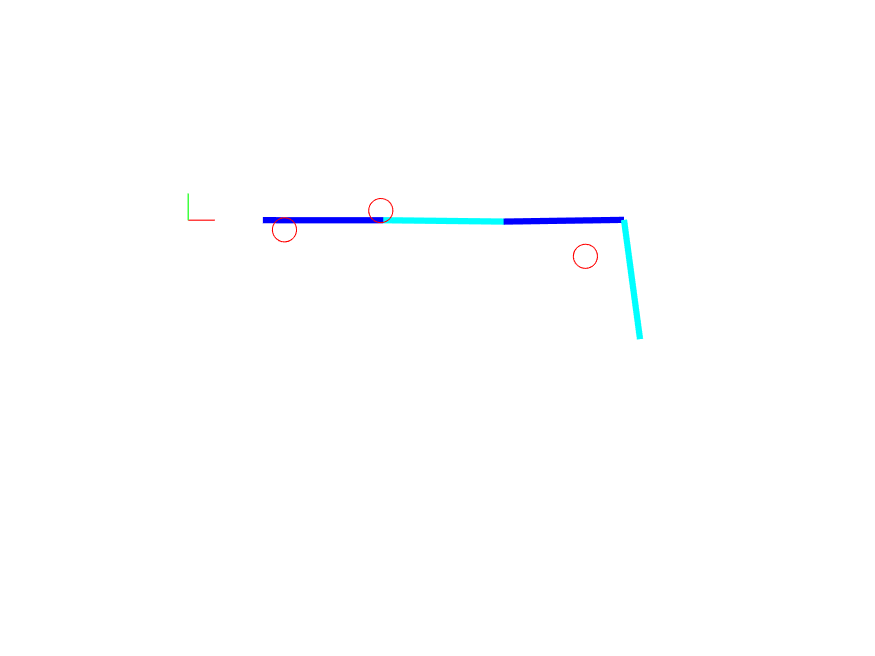
\includegraphics[trim=2cm 4cm 2cm 1.5cm, clip=true, totalheight=0.18\textheight]{figures/case-2-1/sim5.png}}
    \hfil
    \subfloat[$t = 20 s$]{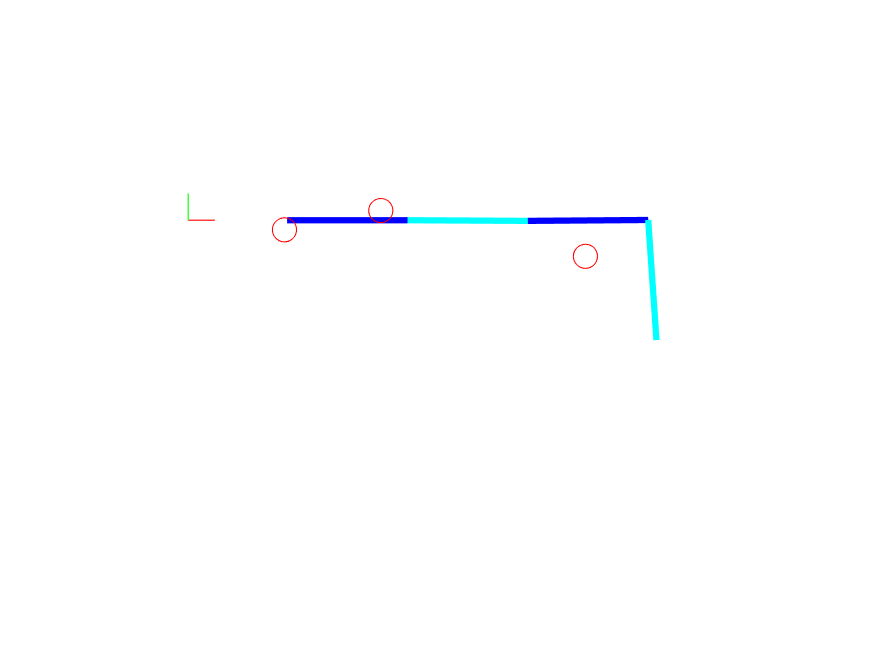
\includegraphics[trim=2cm 4cm 2cm 1.5cm, clip=true, totalheight=0.18\textheight]{figures/case-2-1/sim6.png}}

    \caption{Simulation demo - propulsion with static joint setpoint}
    \label{fig:case2-1}
\end{figure}

From the plots in figure \ref{fig:case2-1-plot} it is clear that the collision with the lower obstacle takes place at \textasciitilde{} 3 seconds. At this point, the joint velocities are projected such that the front link moves to the edge of the obstacle. Additionally, the preceding joints experience an offset as the front joint applies a torque that influences the whole robot.

A repercussion of the geometrical approximation of the contact forces becomes obvious in this experiment. The joint velocities in the emphasised time span in part (b) of figure \ref{fig:case2-1-plot} admit a twitching behaviour as a result of the velocity projections. This circumstance is discussed in chapter \ref{ch:discussion}.

\begin{figure}
    \centering
    
    \subfloat[]{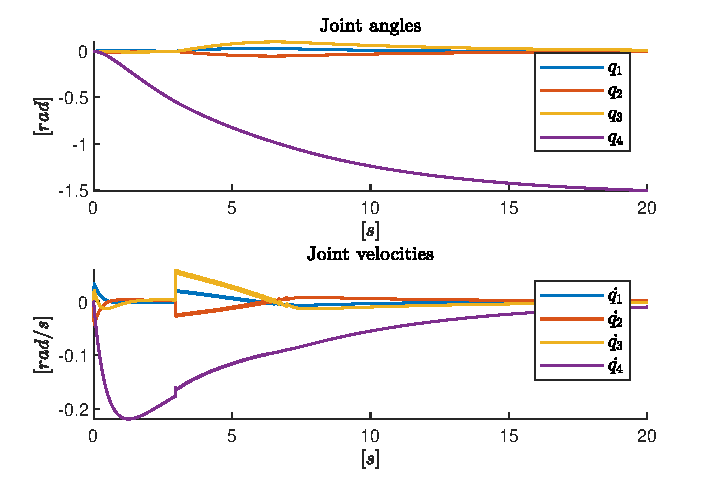
\includegraphics[clip=true, totalheight=0.39\textheight]{figures/case-2-1/case21.pdf}}

    \subfloat[Zoom of joint velocities in seconds 5-10]{\fbox{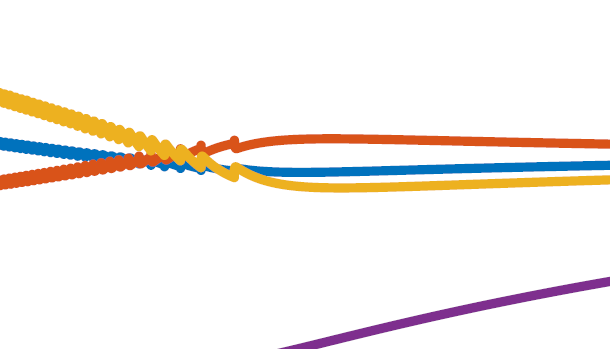
\includegraphics[clip=true, totalheight=0.18\textheight]{figures/case-2-1/zoom21.PNG}}}

    \caption{Joint- angles and velocities for the single setpoint scenario}
    \label{fig:case2-1-plot}
\end{figure}

%---------------------------------------------------------------------------------------
%---------------------------------------------------------------------------------------

\subsection{Case 2.2: No propulsion}\label{subseq:case22}

As propulsion requires a force in the respective direction, there are scenarios where a set of joint torques are insufficient for attaining this force. This scenario aims at illustrating the case where the forces applied work against each other in the direction of propulsion and the robot is simply deformed. The variable configuration for the simulation is presented in table \ref{tab:var-case-2-2} and figure \ref{fig:case2-2} shows a sequence of the motion.

\begin{table}
\centering
    \begin{tabular}{|c|c|c|}
        \hline
         \textbf{Description} & \textbf{Variable name} & \textbf{Value} \\
         \hline
         Simulation time $[s]$& \texttt{simTime} & $9$ \\
         \hline
         Simulation sample time $[s]$ & \texttt{h} & $0.001$ \\
         \hline
         Damping ratio & \texttt{zeta} & $1$ \\
         \hline
         Number of links & \texttt{n} & $3$ \\
         \hline
         Joint angle setpoints $[rad]$& \texttt{q\char`_ref} & $[0, -\pi/3, \pi/3]$ \\
         \hline
         Initial joint angles $[rad]$& \texttt{q\char`_0} & $[0, 0, 0]$ \\
         \hline
         Number of obstacles & \texttt{num\char`_obstacles} & $3$ \\         
         \hline
         Obstacle positions $[m]$& \texttt{obstacle\char`_coords} & \makecell{$(0.5, 0.1)$ \\ $(1.5, -0.1)$ \\ $(2.5, 0.1)$} \\
         \hline
    \end{tabular}
    \caption{Simulation configuration for case 2.2}
    \label{tab:var-case-2-2}
\end{table}


\begin{figure}
    \centering
    
    \subfloat[$t = 0 s$]{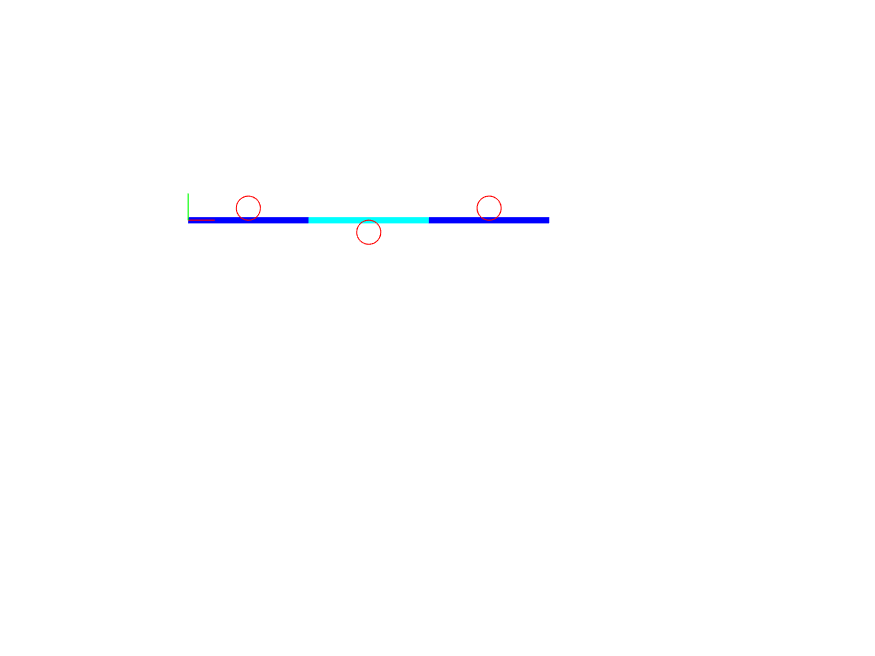
\includegraphics[trim=2cm 4cm 2cm 1.5cm, clip=true, totalheight=0.18\textheight] {figures/case-2-2/2sim1.png}}
    \hfil
    \subfloat[$t = 3 s$]{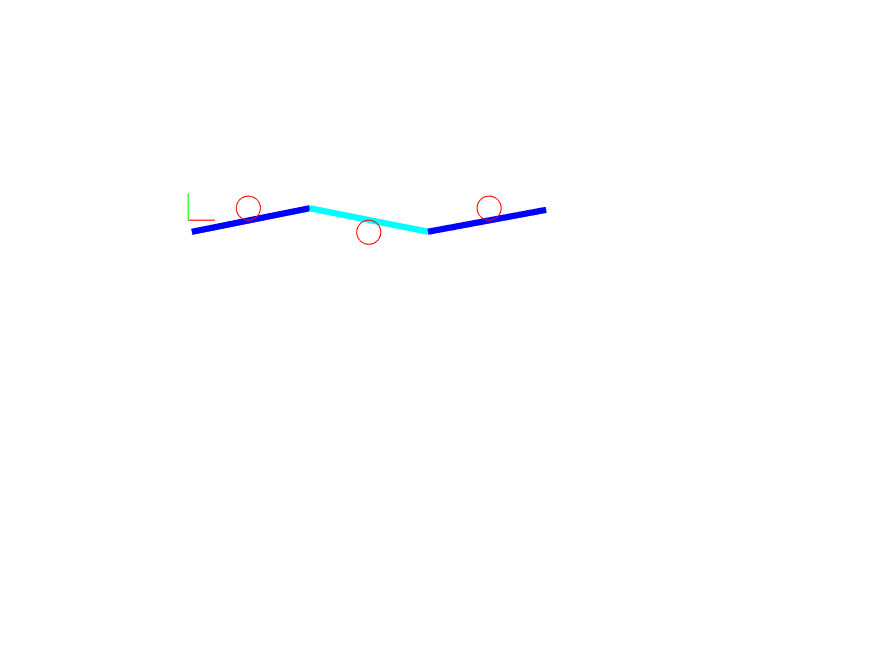
\includegraphics[trim=2cm 4cm 2cm 1.5cm, clip=true, totalheight=0.18\textheight]{figures/case-2-2/2sim2.png}}
    
    \subfloat[$t = 6 s$]{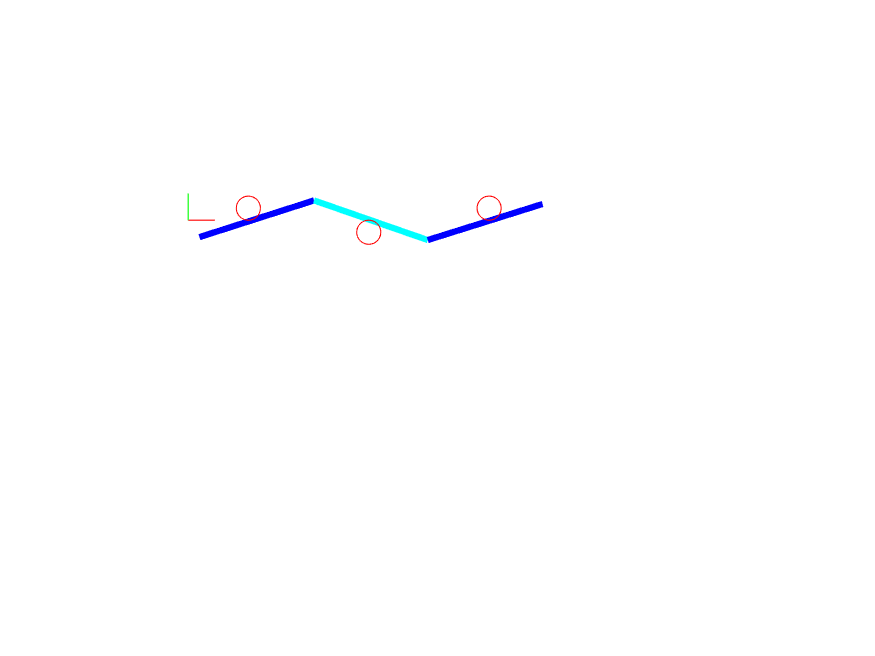
\includegraphics[trim=2cm 4cm 2cm 1.5cm, clip=true, totalheight=0.18\textheight]{figures/case-2-2/2sim3.png}}
    \hfil
    \subfloat[$t = 9 s$]{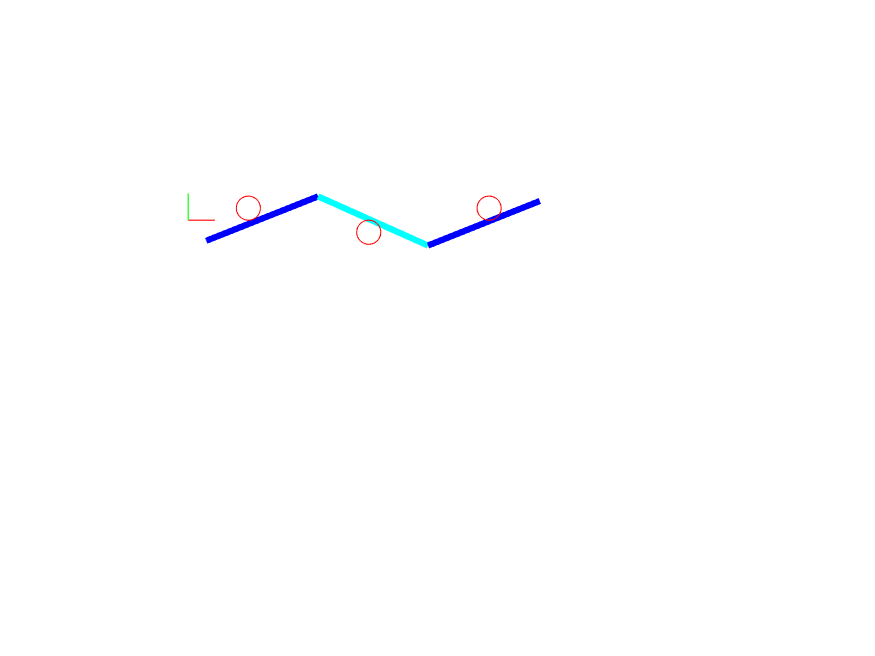
\includegraphics[trim=2cm 4cm 2cm 1.5cm, clip=true, totalheight=0.18\textheight]{figures/case-2-2/2sim4.png}}
    
    \caption{Simulation demo - no propulsion}
    \label{fig:case2-2}
\end{figure}

%---------------------------------------------------------------------------------------
%---------------------------------------------------------------------------------------

\subsection{Case 2.3: Propulsion along path}\label{subseq:case23}

This case is to illustrate how the robot can aid obstacles to propel along a defined path. Since the robot is only position controlled based on deviation from the path, the obstacles are placed in a manner that supports both the desired shape and motion. This configuration can be seen in figure \ref{}. The two obstacles in the back are to keep the rear links on the path, while the obstacle in front is placed so that the robot can push against it and pull itself forward. In order for this to happen, the obstacle has been placed slightly on the path, leading to a constant error from the path. The robot's desire to always stay as close to the path as possible makes it push against the obstacle.

The variable configurations are presented in table \ref{tab:var-case-2-3}. The desired path (\ref{eq:path}) is the same one as in \ref{subseq:case12}.


\begin{table}
\centering
    \begin{tabular}{|c|c|c|}
        \hline
         \textbf{Description} & \textbf{Variable name} & \textbf{Value} \\
         \hline
         Simulation time $[s]$ & \texttt{simTime} & $240$ \\
         \hline
         Simulation sample time $[s]$ & \texttt{h} & $0.001$ \\
         \hline
         Damping ratio & \texttt{zeta} & $1$ \\
         \hline
         Number of links & \texttt{n} & $5$ \\
         \hline
         Joint angle setpoints $[rad]$& \texttt{q\char`_ref} & From path \\
         \hline
         Initial joint angles $[rad]$ & \texttt{q\char`_0} & $[0, 0, 0, 0, 0]$ \\
         \hline
         Number of obstacles & \texttt{num\char`_obstacles} & $3$ \\         
         \hline
         Obstacle positions $[m]$& \texttt{obstacle\char`_coords} & \makecell{$(0.8, -0.1)$ \\ $(1.6, 0.1)$ \\ $(3.2, -0.35)$} \\
         \hline
    \end{tabular}
    \caption{Simulation configuration for case 2.3}
    \label{tab:var-case-2-3}
\end{table}

The movement, as well as the desired path (red), is shown in figure \ref{fig:case2-3}. It is clear that when the robot loses contact with the environment (at approximately 200 seconds), it has trouble with staying close to the path. Keep in mind that all movement is frictionless and that the robot therefore may keep on moving in a direction without simultaneously applying a force to the environment.

Robot moving slightly through obstacle radius towards the end.

\begin{figure}
    \centering
    
    \subfloat[$t = 0 s$]{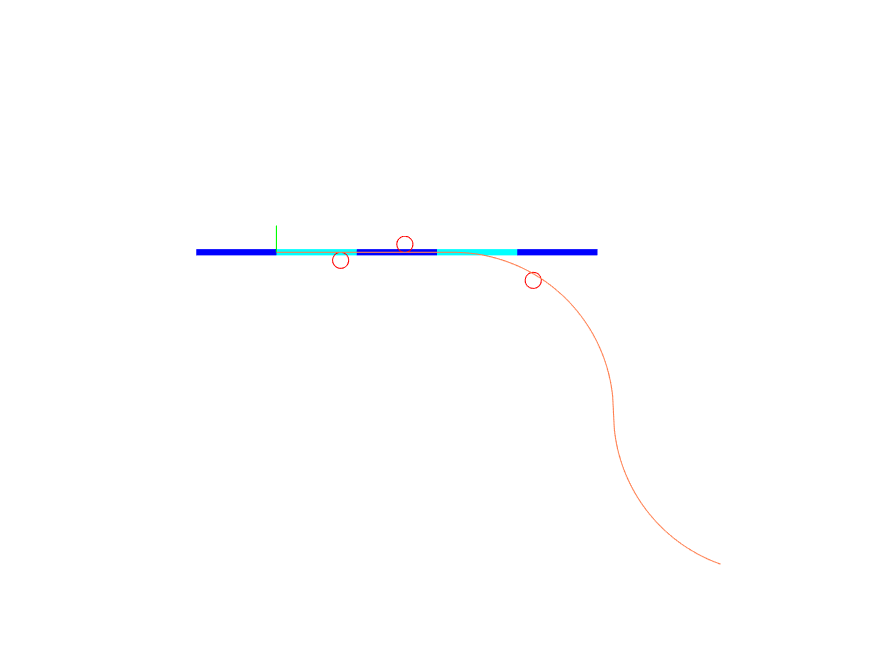
\includegraphics[trim=2cm 3cm 2cm 3cm, clip=true, totalheight=0.15\textheight] {figures/case-2-3/sim1.png}}
    \hfil
    \subfloat[$t = 40 s$]{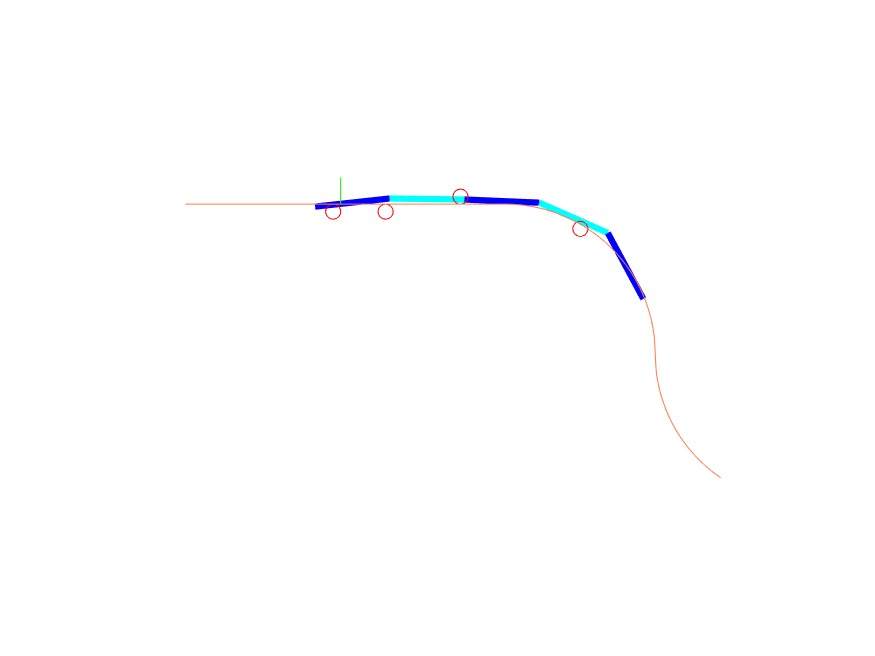
\includegraphics[trim=2cm 3cm 2cm 3cm, clip=true, totalheight=0.15\textheight]{figures/case-2-3/sim3.png}}
    
    \subfloat[$t = 80 s$]{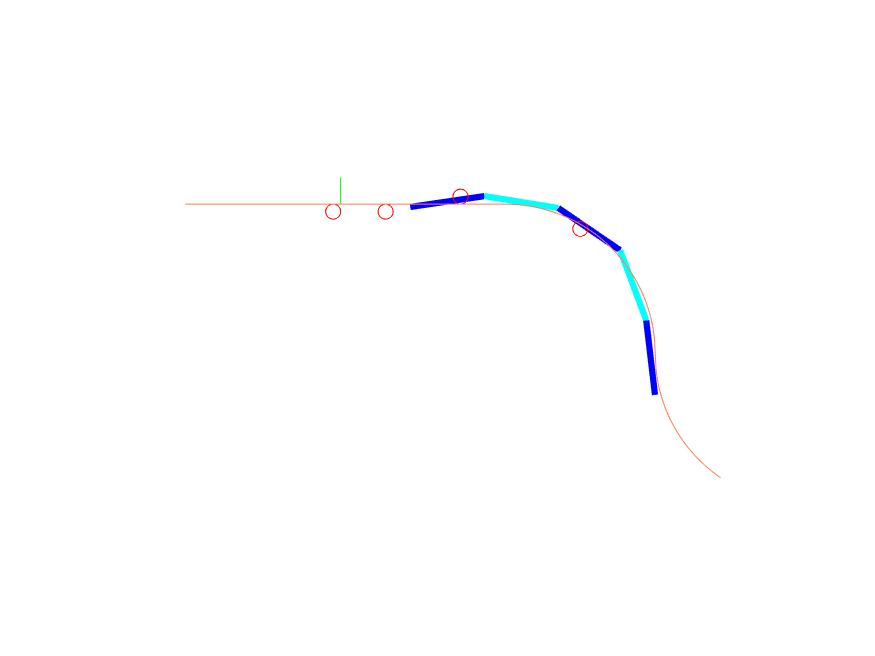
\includegraphics[trim=2cm 3cm 2cm 3cm, clip=true, totalheight=0.15\textheight]{figures/case-2-3/sim5.png}}
    \hfil
    \subfloat[$t = 120 s$]{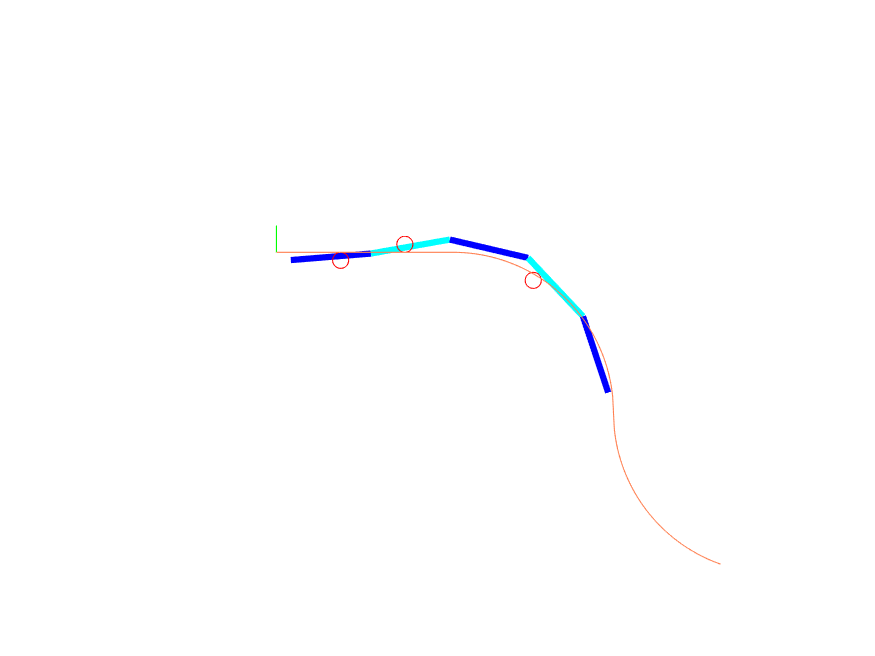
\includegraphics[trim=2cm 3cm 2cm 3cm, clip=true, totalheight=0.15\textheight]{figures/case-2-3/sim7.png}}

    \subfloat[$t = 160 s$]{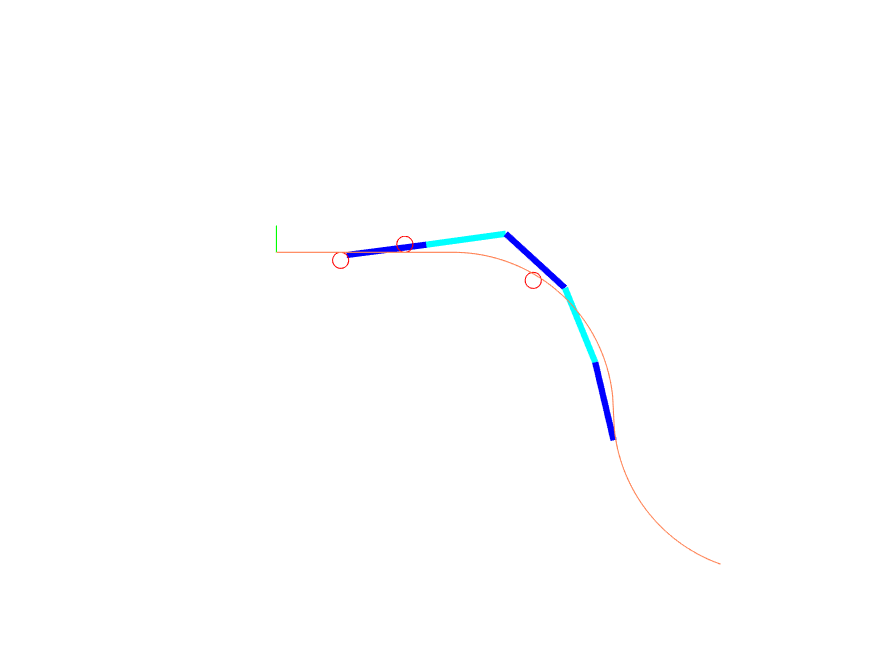
\includegraphics[trim=2cm 3cm 2cm 3cm, clip=true, totalheight=0.15\textheight]{figures/case-2-3/sim9.png}}
    \hfil
    \subfloat[$t = 200 s$]{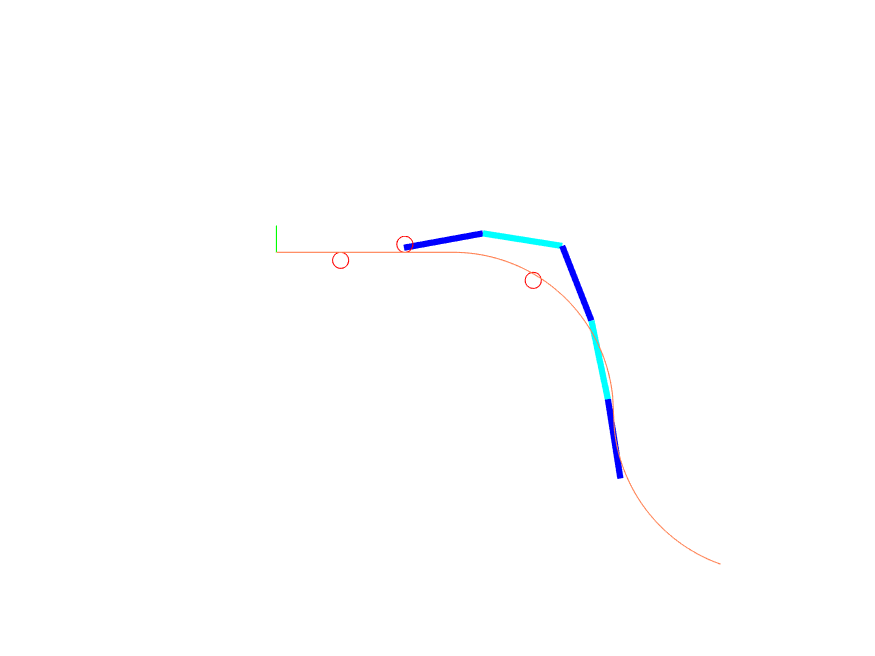
\includegraphics[trim=2cm 3cm 2cm 3cm, clip=true, totalheight=0.15\textheight]{figures/case-2-3/sim92.png}}
    
    \subfloat[$t = 220 s$]{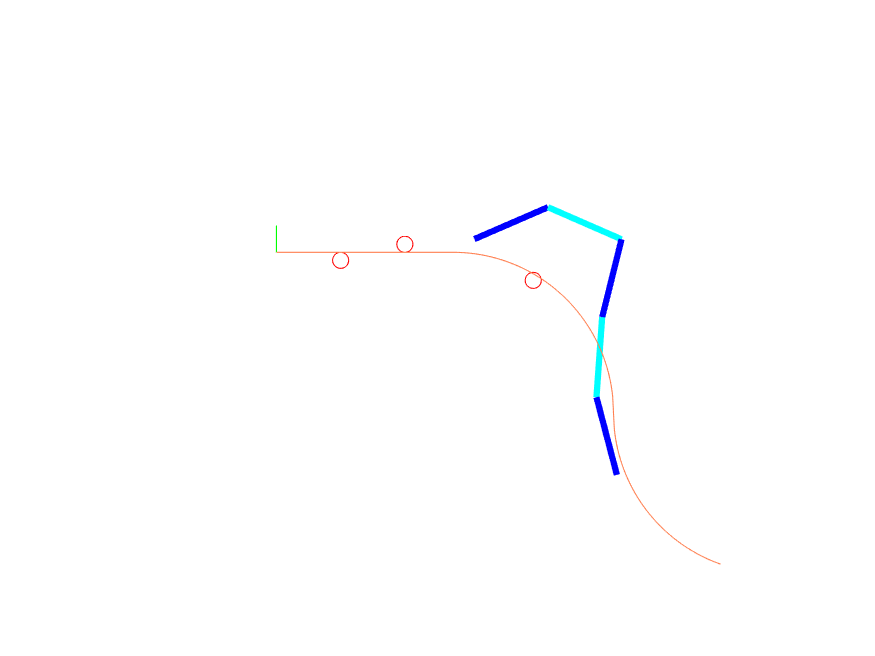
\includegraphics[trim=2cm 3cm 2cm 3cm, clip=true, totalheight=0.15\textheight]{figures/case-2-3/sim94.png}}
    \hfil

    \caption{Simulation demo - propulsion along path}
    \label{fig:case2-3}
\end{figure}

%---------------------------------------------------------------------------------------
%---------------------------------------------------------------------------------------

\subsection{Case 2.4: Unsuccessful propulsion attempt along path}
Robot går baklengst.
Vis sekvens. Plot av posisjon til hodet og path.
Kanskje det funker på samme scenario som simple propulsion, bare med hindringene på andre posisjoner.

%---------------------------------------------------------------------------------------
%---------------------------------------------------------------------------------------
%---------------------------------------------------------------------------------------

